\documentclass[12pt]{article}
\usepackage[brazil]{babel}
\usepackage[T1]{fontenc}
\usepackage{ae}
\usepackage[utf8]{inputenc}
\usepackage{graphicx}
\usepackage{indentfirst}
\usepackage{comment}
\title{Zika PET - PET Shop}
\author{
	João P. de Oliveira,
    \and
    Matheus P. Reis,
    \and
    Gabriel P. Haddad
    \and
    Higor E. de Souza
}

\begin{document}
  \maketitle               %título
  \newpage                 %quebra de página

\begin{comment}
  \tableofcontents         %Sumário
  \newpage                 %quebra de página
       
  \listoffigures           %Lista de figuras
  \newpage 
\end{comment}
 
 %Documento
 \section{Descrição geral do problema}
 Consiste na criação de um sistema de pet shop que efetue venda de produtos, consulta veterinária, hospedagem do animal do cliente e cuidados com os animais.
 
 O cliente efetua o cadastro juntamente com seu animal. Ele pode efetuar compras para seu animal, alugar uma hospedagem e fazer uma consulta. A consulta pode resultar em um encaminhamento à uma lista de clínicas veterinárias que externas ao Zika pet, para encaminhamentos como cirurgia, exames, etc. 
 O Cliente também tem a opção de fazer uma hospedagem, e em seguida, realizar um cuidado. Os cuidados podem ser um banho ou uma tosa 
 Um animal pode ser do tipo gato ou cachorro. Ele se cadastra juntamente com o  dono e está associado a consulta, hospital e cuidados
 
 Os indivíduos são diferenciados pelo CPF, e o animal pelo seu nome e dono. Os funcionários podem ser:
 
\begin{enumerate}
\item \textbf{Atendente:} Fica por conta das vendas, e dos cadastros.

\item \textbf{Veterinário:} Realiza as consultas e os encaminhamentos, se necessário.

\item \textbf{Cuidador:} Cuida dos serviços de hospedagem e cuidados com o animal.

\item \textbf{Gerente:} O gerente fica apenas na parte de vendas, se o funcionário não consegue atender à solicitação, ele à envia ao gerente, faz também o . Além fazer o cadastro dos funcionários
\end{enumerate}
 
 \section{Requisitos funcionais}%Principais funcionalidades a serem implementadas
 Cadastro de clientes, animais e funcionários. Fará a administração do pet shop registrando todos os animais e clientes que passaram pelo Zika pet shop a fim de fazer controle e armazenamento de dados de forma segura através de um banco de dados.
 
 
 \section{Requisitos não funcionais}%Restrições de implementação/uso do sistema 
 A segurança de login de usuários será feita pelo PostgreeSQL que será o BD(Banco de dados) utilizado no projeto, deixando a aplicação livre da autenticaçãoe da durabilidade de dados. Como o programa vai ser feito em Java, o usuário deve ter a JVM(Java virtual machine) instalada em uma máquina com o SO Windows 10.
 
 O hardware utilizado foi um notebook Lenovo Y720 com processador Intel core i7 7700 HQ, com 16BG de memória principal e placa de vídeo NVIDIA GTX 1060.
 
 

 \section{Diagrama de classes}
 \begin{flushleft}
 
 \begin{figure}[!h]
     \centering
     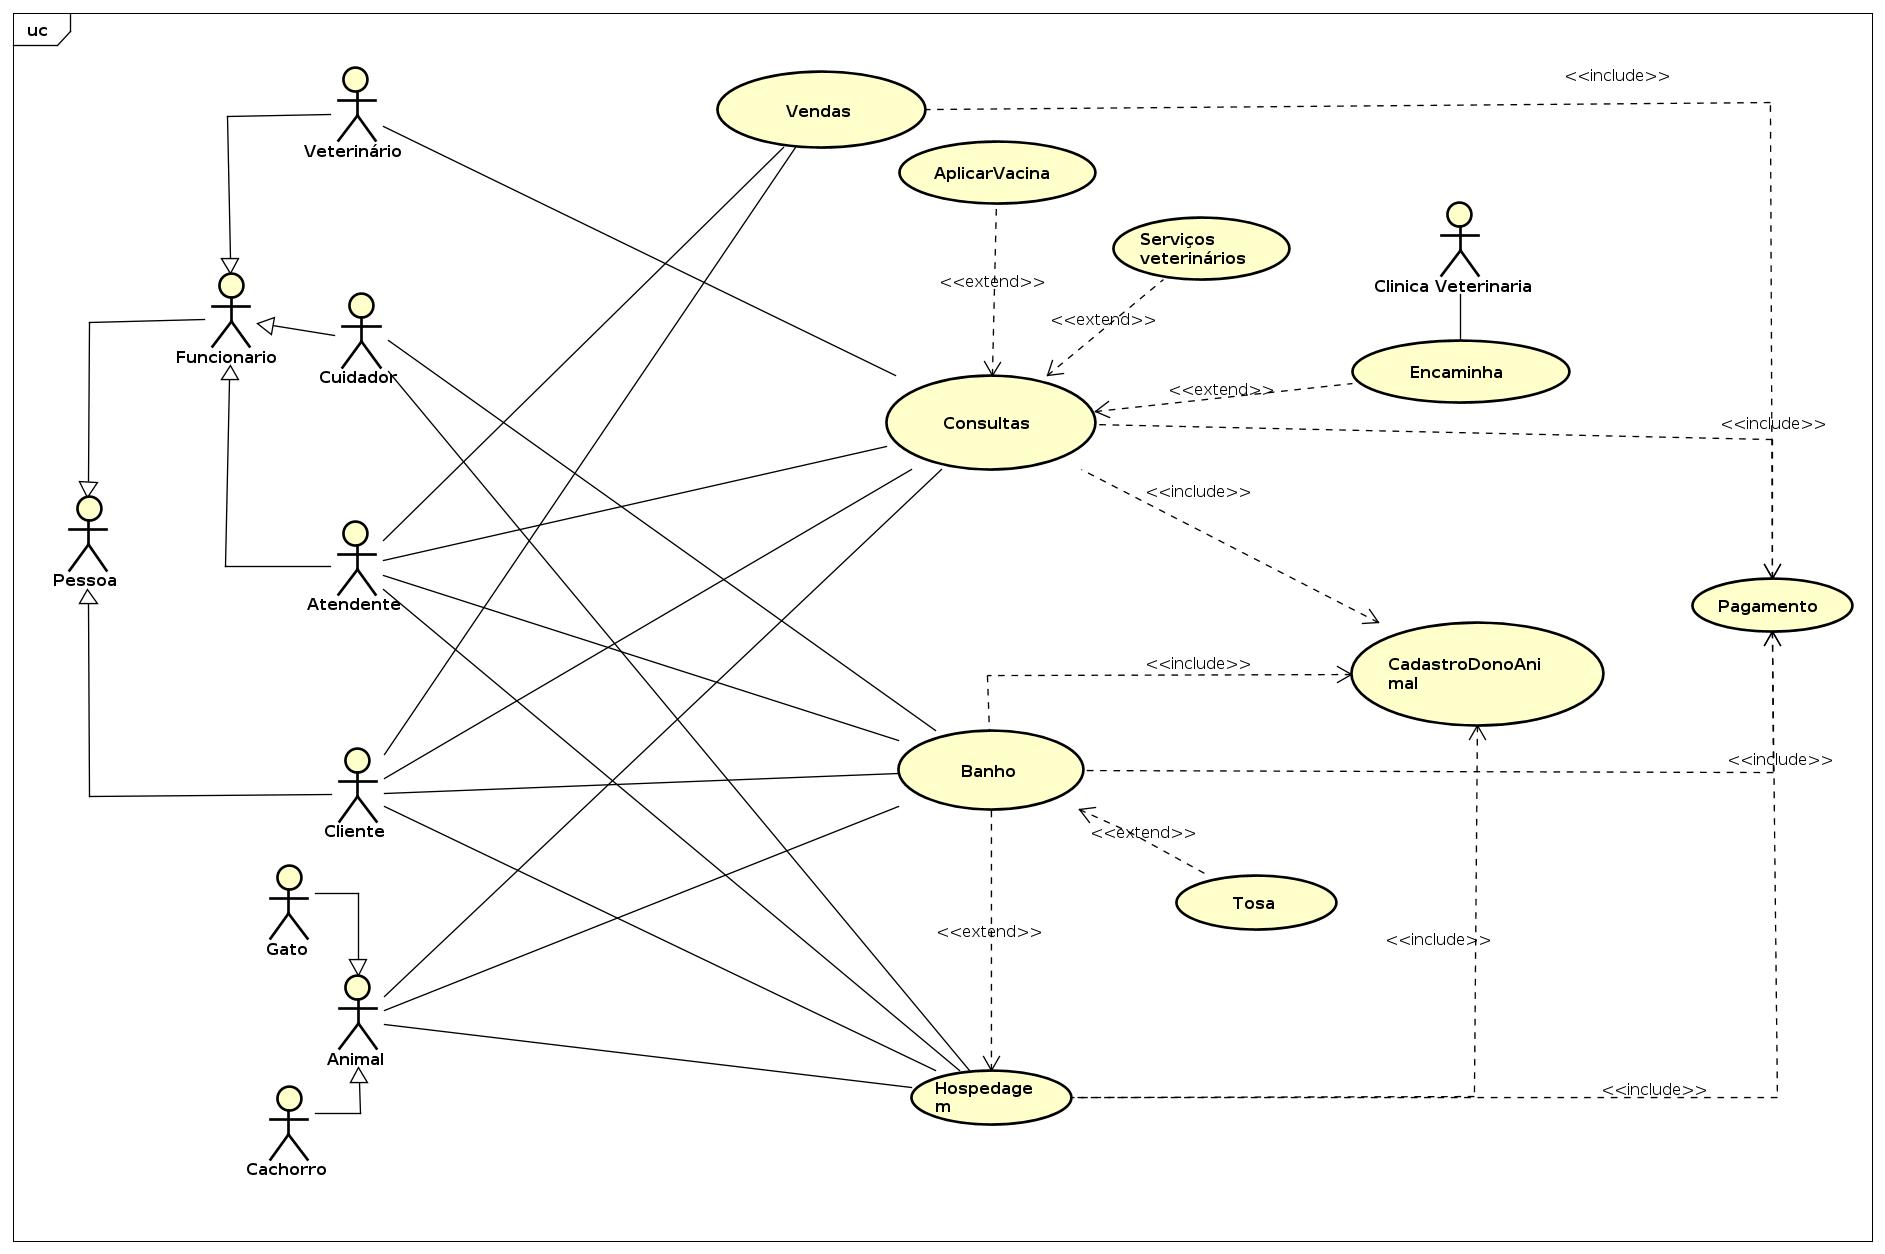
\includegraphics[scale=0.43,angle=90]{Diagrama.jpg}
\end{figure}
 \end{flushleft} 
\end{document}
